\chapter{การวิเคราะห์และออกแบบระบบ}

การวิเคราะห์และการออกแบบแอปพลิเคชันค้นหายาเพื่อคุณ เนื่องจากคณะเภสัชศาสตร์ได้สร้างฐานข้อมูลพิสูจน์เอกลักษณ์ยาเม็ดและแคปซูลในประเทศไว้เรียบร้อย ทางผู้พัฒนาจึงได้ดำเนินการเขียนเว็บเซอร์วิส ใช้สำหรับติดต่อฐานข้อมูลพิสูจน์เอกลักษณ์ยาเม็ดและแคปซูลของคณะเภสัชศาสตร์เพื่อดึงข้อมูลพิสูจน์เอกลักษณ์ยาเม็ดและแคปซูลส่งออกให้แอปพลิเคชันในรูปแบบ JSON และการแผนภาพในการออกแบบระบบมีดังนี้ 
\begin{itemize}[label={--}]
	\item รายละเอียดการออกแบบแอปพลิเคชัน
	\item Use Case Diagram เป็นแผนภาพที่ใช้แสดงให้ทราบว่าระบบทำงานหรือมีหน้าที่ใดบ้าง
	\item Class Diagram เป็นแผนภาพที่ใช้แสดง Class และความสัมพันธ์ระหว่าง Class
	\item Sequence Diagram เป็นแผนภาพที่ใช้แสดงให้เห็นถึงการตอบโต้ข้อมูลระหว่างคลาส เรียงตามลำดับของเวลาที่เกิดเหตุการณ์จากน้อยไปมาก
	\item State Diagram ใช้เพื่อแสดงสถานะของวัตถุ รวมไปถึงเหตุการณ์ในแอปพลิเคชัน
	\item การประมวลผลภาพยาเม็ดเพื่อการพิสูจน์เอกลักษณ์ยาเม็ด
\end{itemize}	

\section{รายละเอียดการออกแบบแอปพลิเคชัน}
	โครงงานแอปพลิเคชันค้นหายาเพื่อคุณ Drugiden แบ่งส่วนการทำงานออกเป็น 2 ส่วนหลัก ได้แก่ ส่วนแอปพลิเคชัน และส่วนเว็บเซอร์วิส
	\begin{figure}
		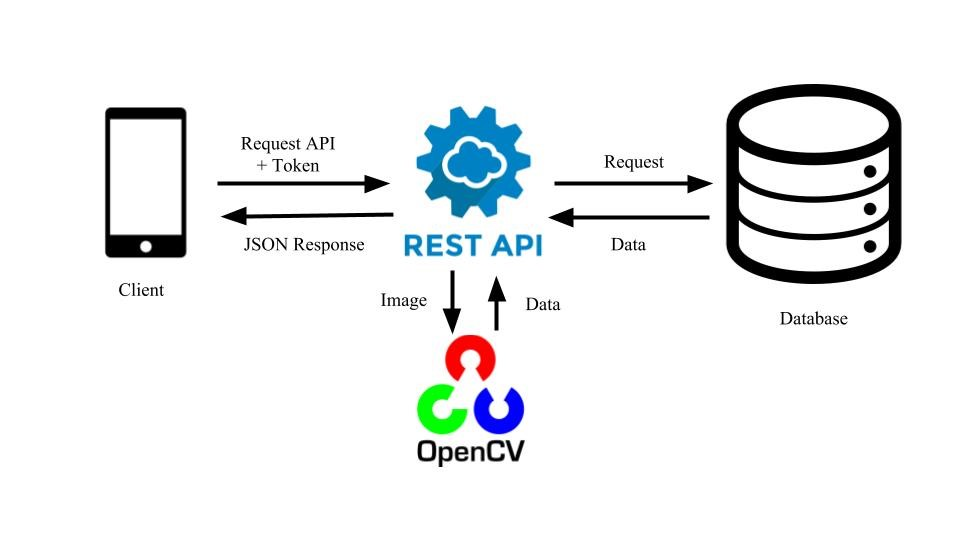
\includegraphics[width=\columnwidth]{Figures/3/project-structure}
		\caption{ภาพรวมของแอปพลิเคชันค้นหายาเพื่อคุณ}
		\label{Fig:project-structure}
	\end{figure}
	\subsection{ส่วนแอปพลิเคชัน}

		ส่วนแอปพลิเคชันผู้ใช้งานสามารถใช้งานฟังก์ชันดังต่อไปนี้

	\begin{enumerate}
		\item สามารถค้นหายาเม็ดแบบทั่วไป
		เป็นการค้นหาที่ใช้ key word ในการค้นหา เช่น para, น้ำเงิน, ส้ม, CAPSULE เป็นต้น 
		\item สามารถค้นหายาเม็ดแบบขั้นสูง
		เป็นการค้นหาที่ต้องใช้การระบุเอกลักษณ์ของยาเม็ดหรือแคปซูลแบบเจาะจง ลักษณะทางกายภาพหรือข้อมูลรายละเอียดต่างๆ
		\item สามารถดูรายละเอียดยาเม็ด
		เป็นการดูรายละเอียดของยาเม็ดหรือแคปซูลนั้นๆ ได้ทั้งดูรูปภาพ ข้อมูลยาต่างๆ เช่น ผู้ผลิต ผู้รับอนุญาติ ผู้จำหน่วย ขนาด กว้าง ยาว รูปแบบผลิตภัณฑ์ รูปร่าง ประเภทของยา เป็นต้น
		\item สามารถดูรายการยา
		เป็นการแสดงรายการยาที่เป็นผลลัพธ์จากการค้นหายาเม็ดแบบทั่ว การค้นหายาแบบขั้งสูง และรายการบุ๊กมาร์กยา
		\item สามารถกดบันทึกบุ๊กมาร์กรายการยา
		เพื่อบันทึกลงบนเครื่องผู้ใช้งานและดูย้อนหลังได้
		\item สามารถดูรายการบุ๊กมาร์กยา
		เป็นการดูรายการบุ๊กมาร์กยาที่ผู้ใช้งานกดบันทึกบุ๊กมาร์ก
		\item ถ่ายรูปภาพยาเม็ดเพื่อพิสูจน์เอกลักษณ์ยา
		เป็นการเปิดกล้องเพื่อถ่ายรูปภาพยาเม็ดและส่งรูปภาพไปประมวลผลที่ API service 
	\end{enumerate}

	\subsection{ส่วนเว็บเซอร์วิส}
	เว็บเซอร์วิสใช้เป็นสื่อในการแลกเปลี่ยนข้อมูลกันระหว่างแอปพลิเคชันและฐานข้อมูลในรูปแบบ JSON 
	โดยจะเรียกว่า API (Application Programming Interface) 
	ที่จะคอยกระทำการต่างๆ เช่น การดึงข้อมูลยา การประมวลผลรูปภาพ เป็นต้น 
	และส่วนเว็บเซอร์วิสมีหน้าที่การทำงานดังต่อไปนี้
	\begin{enumerate}
		\item สามารถติดต่อกับฐานข้อมูลการพิสูจน์เอกลักษณ์ยาเม็ดหรือแคปซูลของหน่วยข้อมูลยาและสุขภาพ คณะเภสัชศาสตร์ มหาวิทยาลัยอุบลราชธานี 
		\item สามารถค้นหาเม็ดยากับฐานข้อมูลการพิสูจน์เอกลักษณ์ยาเม็ดหรือแคปซูล 
		โดยการใช้พารามิเตอร์จากการร้องขอทรัพยากร (Request) ของแอปพลิเคชัน เช่น สี รูปทรง ขนาด ชื่อการค้า ชื่อสามัญ เป็นต้น 
		\item สามารถพิสูจน์ตัวตนของผู้ใช้งาน 
		เว็บเซอร์วิสมีการพิสูจน์ตัวตนผู้ใช้งานก่อนเรียกใช้งานการร้องขอด้วย JSON Web Token 
		เพื่อป้องกันการเรียกใช้งานจากผู้ที่ไม่พึ่งประสงค์ 
		\item สามารถถอดรหัสรูปภาพแบบ base64 
		\item สามารถประมวลผลภาพเพื่อหาลักษณะของเม็ดยา 
		ได้แก่ รูปทรง ขนาดและสี 
	\end{enumerate}

\newpage
\section{Use Case Diagram}
	Use Case Diagram เป็นแผนผังเพื่อแสดงฟังก์ชันแสดงการทำงานของระบบโดยรวม แสดงส่วนประกอบในระบบและกิจกรรมที่เกิดขึ้นในระบบ สัญลักษณ์ที่ใช้ในการเขียน Use Case Diagram แสดงในตารางที่ \ref{tab:use-case}

	\begin{table}[H]
		\centering
		\caption{สัญลักษณ์ของ Use case Diagram}
		\label{tab:use-case}
		\begin{tabular}{|c|p{10cm}|}
		\hline
		\textbf{สัญลักษณ์} & \multicolumn{1}{c|}{\textbf{การใช้งาน}} \\ \hline
		\raisebox{-\totalheight}{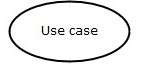
\includegraphics[width=0.3\textwidth]{Figures/table/use-case/1}}
		& \setstretch{1.5} {Use case คือส่วนย่อยของระบบงาน แทนด้วยวงรีและชื่อของ Use case ภายในวงรี} \\ \hline
		\raisebox{-\totalheight}{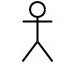
\includegraphics[height=1.5cm]{Figures/table/use-case/2}}
		& \setstretch{1.5} {Actor คือบุคคลหรือระบบงานอื่นที่ใช้งานระบบหรือได้รับประโยชน์จากระบบซึ่งอยู่ภายนอกระบบ แทนด้วยรูปคนและมีชื่อบทบาทการใช้งานระบบ} \\ \hline
		\raisebox{-\totalheight}{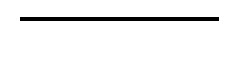
\includegraphics[width=3cm]{Figures/table/use-case/3}}
		& \setstretch{1.5} {เส้นตรงที่แสดงถึงการใช้งาน Use case ของผู้กระทำ} \\ \hline
		\raisebox{-\totalheight}{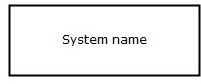
\includegraphics[width=0.3\textwidth]{Figures/table/use-case/4}}
		& \setstretch{1.5} {กรอบสี่เหลี่ยมแสดงถึงขอบเขตของระบบโดยแสดงชื่อระบบภายในหรือด้านบนกรอกสี่เหลี่ยม Use case อยู่ภายในกรอบสี่เหลี่ยม และ actor อยู่ภายนอกกรอบสี่เหลี่ยม} \\ \hline
		\raisebox{-\totalheight}{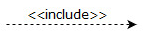
\includegraphics[width=0.3\textwidth]{Figures/table/use-case/5}}
		& \setstretch{1.5} {ความสัมพันธ์แบบ <<includes>> แสดงว่า Use case หนึ่งดำเนินการตามขั้นตอนของ Use case อื่น โดยแทนด้วยสัณลักษณ์ลูกศรเส้นประ ซึ่ง Use case ที่หางลูกศรเรียกใช้งาน Use case ที่หัวลูกศรทุกครั้งที่มีการทำงาน} \\ \hline
		\raisebox{-\totalheight}{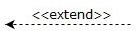
\includegraphics[width=0.3\textwidth]{Figures/table/use-case/6}}
		& \setstretch{1.5} {ความสัมพันธ์แบบ <<extend>> แสดงว่า Use case หนึ่งดำเนินการตามขั้นตอนของ Use case อื่น โดยแทนด้วยสัญลักษณ์ลูกศรเส้นประ ซึ่ง Use case ที่หัวลูกศรเรียกใช้งาน Use case ที่หางลูกศร แต่การใช้งานไม่จำเป็นต้องเกิดขึ้นทุกครั้งขึ้นอยู่กับเงื่อนไขระหว่างการทำงาน} \\ \hline
		\end{tabular}
	\end{table}

	\begin{figure}[H]
		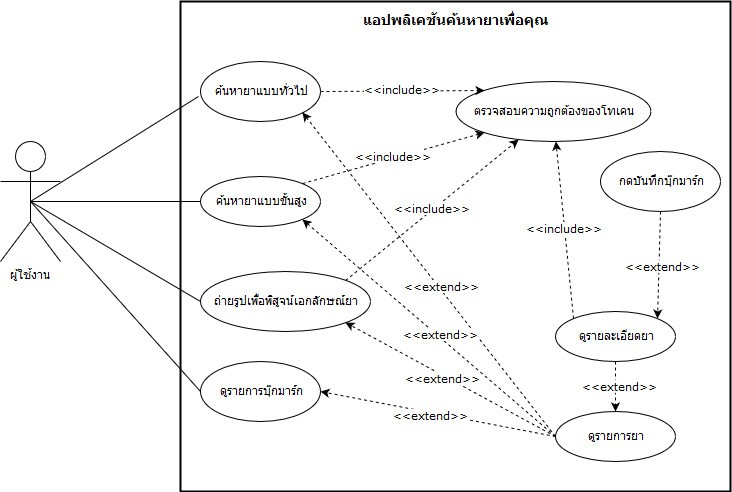
\includegraphics[width=\columnwidth]{Figures/3/case-use}
		\caption{Use Case Diagram ของแอปพลิเคชันค้นหายาเพื่อคุณ}
		\label{Fig:case-use}
	\end{figure}
	ในการพัฒนาแอปพลิเคชันค้นหายาเพื่อคุณสามารถอธิบายขั้นตอนการทำงานที่สำคัญและความสัมพันธ์ต่างๆ ของระบบด้วย Use Case Diagram แสดงดังรูปที่ \ref{Fig:case-use} ซึ่งประกอบด้วย Use case ต่างๆ ดังนี้

	\begin{enumerate}
		\item ค้นหายาแบบทั่วไป : ทำหน้าที่การสืบค้นแบบให้ผู้ใช้งานกรอกคำสำคัญ เช่น ชื่อบริษัท ชื่อการค้า รูปร่าง สี ขนาด เป็นต้น
		\item ค้นหายาแบบขั้นสูง : ทำหน้าที่การสืบค้นแบบให้ผู้ใช้งานกรอกรายละเอียดของยาเม็ด เช่น รูปร่าง สี ขนาด เป็นต้น
		\item ถ่ายรูปเพื่อพิสูจน์เอกลักษณ์ยา : ทำหน้าที่ให้ผู้ใช้งานถ่ายรูปภาพยาเม็ดเพื่อการพิสูจน์เอกลักษณ์ยาเม็ด
		\item ดูรายการยา : ทำหน้าที่แสดงรายการยาจากการค้นหายาแบบทั่วไป ค้นหายาแบบขั้นสูง การถ่ายรูปเพื่อพิสูจน์เอกลักษณ์ยา และการดูรายการบุ๊กมาร์ก
		\item ดูรายละเอียดยา : ทำหน้าที่แสดงรายละเอียดของยาเม็ดให้แก่ผู้ใช้งาน
		\item กดบันทึกบุ๊กมาร์กยา : ทำหน้าที่บันทึกรายการยาเอาไว้ในเครื่องผู้ใช้งาน
		\item ดูรายการบุ๊กมาร์ก : ทำหน้าที่แสดงรายการบุ๊กมาร์กทั้งหมดที่ผู้ใช้กดบันทึกในเครื่องผู้ใช้งาน
		\item ตรวจสอบความถูกต้องของโทเคน : ทำหน้าที่ตรวจสอบความถูกต้องของโทเคนของแอปพลิเคชันกับเว็บเซอร์วิส ก่อนจะสามารถใช้งานแอปพลิเคชั่นได้
	\end{enumerate}

\newpage
\section{Class Diagram}
	Class Diagram คือแผนภาพที่ใช้แสดงคลาสและความสัมพันธ์ในแบบต่างๆ ระหว่างคลาส สัญลักษณ์ที่ใช้ในการเขียน Class Diagram แสดงในตารางที่ \ref{tab:class} 
	\begin{center}
	\begin{table}[H]
		\centering
		\caption{สัญลักษณ์ของ Class Diagram}
		\label{tab:class}
		\begin{tabular}{|c|p{10cm}|}
		\hline
		\textbf{สัญลักษณ์} & \multicolumn{1}{c|}{\textbf{การใช้งาน}} \\ \hline
		\raisebox{-\totalheight}{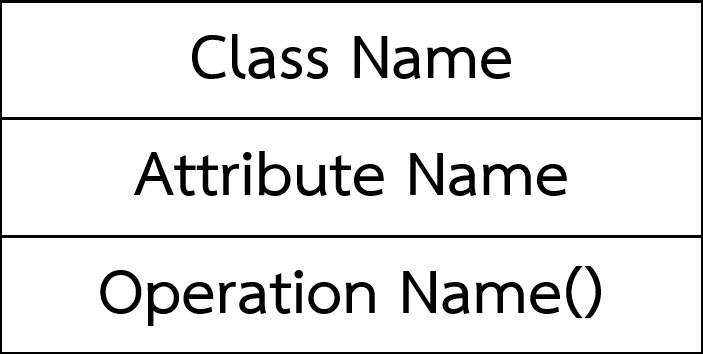
\includegraphics[width=0.3\textwidth]{Figures/table/class/11}}
		& \setstretch{1.5} {Class สัญลักษณ์แทนด้วยสี่เหลี่ยมแบ่งเป็น 3 ส่วน ส่วนบนเป็นชื่อ Class ส่วนกลางเป็น Attribute และส่วนล่างเป็น Operation Name หรือ Method ซึ่งคลาสเป็นสิ่งที่เก็บรวบรวมข้อมูลที่แสดงถึงบุคคล สถานที่ เหตุการณ์หรือสิ่งต่างๆ ที่มีความเกี่ยวข้องกับระบบ Method เป็นการกระทำหรือฟังก์ชันที่คลาสนั้นสามารถทำได้} \\ \hline
		Method Name()
		& \setstretch{1.5} {Method สามารถแบ่งการมองเห็น (Visibility) ได้ 3 ชนิดได้แก่ 
			\begin{enumerate}
				\item Public แทนสัญลักษณ์ด้วยเครื่องหมายบวก (+)
				\item Private แทนสัญลักษณ์ด้วยเครื่องหมายบวก (-)
				\item Protected แทนสัญลักษณ์ด้วยเครื่องหมายบวก (\#)
			\end{enumerate}
		} \\ \hline
		\raisebox{-\totalheight}{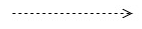
\includegraphics[width=0.3\textwidth]{Figures/table/class/1}}
		& \setstretch{1.5} {Dependency Relationship หมายความว่า คลาสที่อยู่ฝั่งต้นลูกศรสามารถเรียกใช้คลาสที่อยู่ฝั่งหัวลูกศร} \\ \hline
		\raisebox{-\totalheight}{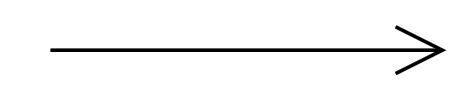
\includegraphics[width=0.3\textwidth]{Figures/table/class/4}}
		& \setstretch{1.5} Generalization หมายความว่า คลาสที่อยู่ฝั่งต้นลูกศรทำการสืบทอดคลาสที่อยู่หัวลูกศร} \\ \hline
		\raisebox{-\totalheight}{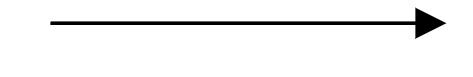
\includegraphics[width=0.3\textwidth]{Figures/table/class/5}}
		& \setstretch{1.5} {Association Relationship หมายความว่า คลาสที่อยู่ฝั่งต้นลุกศรทำการกำหนดคลาสอื่นในรูป Attribute ภายในคลาส และสามารถเรียกใช้ Method จากคลาสนั้นได้} \\ \hline
		\end{tabular}
	\end{table}
	\end{center}
	% \begin{table}[H]
	% 	\caption{สัญลักษณ์ของ Class Diagram}
	% 	\label{tab:class}		
	% 	\begin{tabular}{c}
	% 		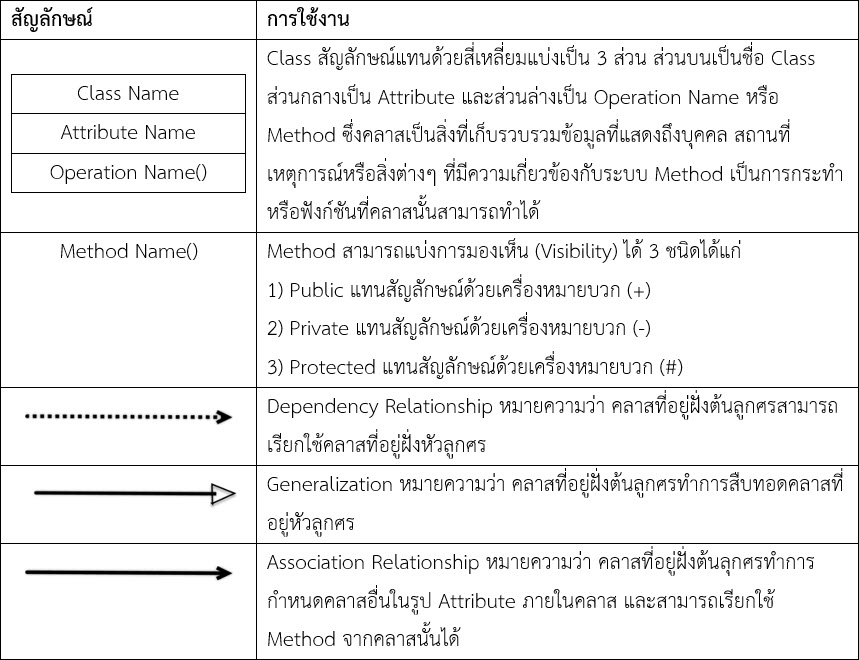
\includegraphics[width=\columnwidth]{Figures/table/class}	\\ 
	% 	\end{tabular}
	% \end{table}

	Class Diagram แสดงความสัมพันธ์ในรูปแบบต่างๆ ระหว่างคลาสของแอปพลิเคชันค้นหายาเพื่อคุณ อธิบายได้ตามรูปที่ \ref{Fig:class} ดังต่อไปนี้

	\begin{figure}[H]
		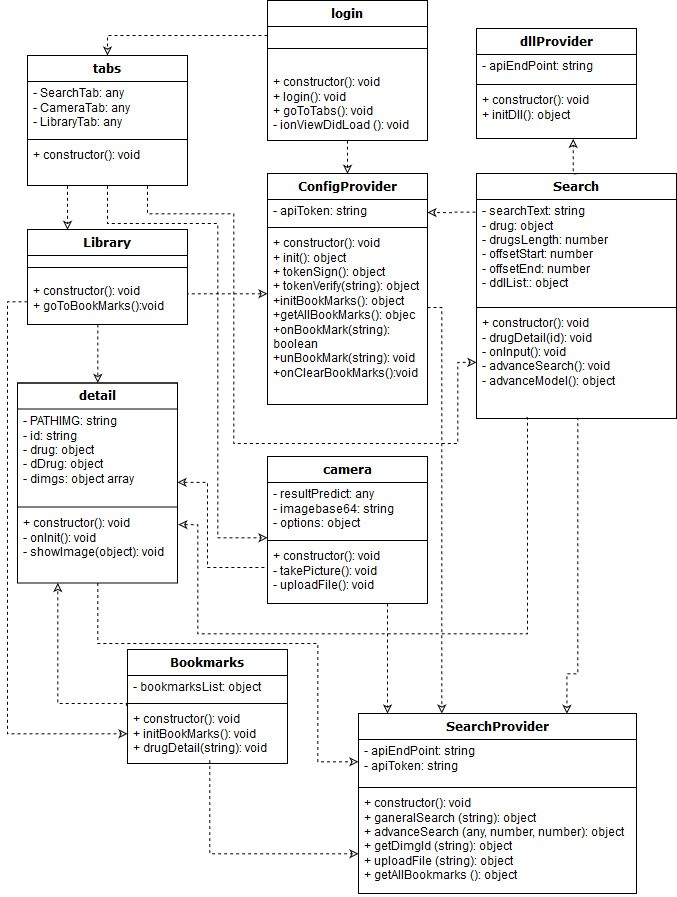
\includegraphics[width=\columnwidth]{Figures/3/class}
		\caption{Class Diagram ของแอปพลิเคชันค้นหายาเพื่อคุณ}
		\label{Fig:class}
	\end{figure}

	\newpage
	จากรูปที่ \ref{Fig:class} สามารถอธิบายแผนภาพ Class Diagram ได้ดังต่อไปนี้
	\begin{enumerate}
		\item Class Login เป็นคลาสที่แสดงหน้าแรกของแอปพลิเคชัน เพื่อเข้าสู่ระบบอัตโนมัติโดยจะทำงานร่วมกันคลาส ConfigProvider สำหรับการตรวจสอบความถูกต้องของโทเคนหรือการร้องขอโทเคนจากเว็บเซอร์วิสในการใช้แอปพลิเคชัน 
		\item Class Tabs เป็นคลาสที่จัดการและแสดงหน้าแท็บทั้ง 2 คลาส ได้แก่ คลาส Search และคลาส Camera 
		\item Class ConfigProvider เป็นคลาสที่กำหนดค่าเริ่มต้นของแอปพลิเคชัน ได้แก่ การร้องขอโทเคนจากเว็บเซอร์วิส และการตรวจสอบความถูกต้องของโทเคน 
		\item Class Camera เป็นคลาสที่เปิดการทำงานของกล้องถ่ายรูปเพื่อให้ถ่ายรูปและประมวลผลภาพ
		\item Class Search เป็นคลาสที่แสดงหน้าการค้นหายาแบบทั่วไปและการค้นหายาแบบละเอียด โดยจะทำงานร่วมกับคลาส SearchProvider สำหรับใช้ร้องขอไปที่เว็บเซอร์วิสเพื่อค้นหายา และทำงานร่วมกับคลาส dllProvider สำหรับใช้ร้องขอไปที่เว็บเซอร์วิสเพื่อดึงรายการ dropdown มาแสดง
		\item Class Library เป็นคลาสที่แสดงรายการคำสั่งในการจัดการกับรายการบุ๊กมาร์กยา 
		\item Class Bookmarks เป็นคลาสที่แสดงรายการบุ๊กมาร์กของผู้ใช้งานที่ถูกเก็บไว้ในเครื่องผู้ใช้งาน 
		\item Class SearchProvider เป็นคลาสที่จัดการการเชื่อมต่อกับเว็บเซอร์วิส ได้แก่ การร้องขอไปยังเว็บเซอร์วิสเพื่อการค้นหาทั่วไปกับการค้นหาแบบละเอียด การร้องขอไปยังเว็บเซอร์วิสเพื่อการดึงข้อมูลยาแบบละเอียด
		\item Class Detail เป็นคลาสที่แสดงข้อมูลยาแบบละเอียดที่ได้มาจากคลาส SearchProvider 
		\item Class dllProvider เป็นคลาสที่จัดการกับรายการ dropdown ที่ร้องข้อไปยังเว็บเซอร์วิส 
	\end{enumerate}

\newpage
\section{Sequence Diagram}
	Sequence Diagram เป็น Diagram ที่แสดงขั้นตอนการทำงานของแต่ละ Use Case ระหว่าง Object ต่างๆ ที่ส่งข้อความถึงกันและกัน โดย Sequence Diagram จะช่วยให้มองเห็นการทำงานของภาพรวมของระบบ ส่วนประกอบสัญลักษณ์ที่ใช้ในการเขียน Sequence Diagram 
	แสดงดังตารางที่ \ref{tab:Sequences}
	
	\begin{table}[H]
		\centering
		\caption{สัญลักษณ์ของ Sequence Diagram}
		\label{tab:Sequences}
		\begin{tabular}{| c	| p{10cm} |}
		\hline
		\textbf{สัญลักษณ์} & \multicolumn{1}{c|}{\textbf{การใช้งาน}} \\ \hline
		\raisebox{-\totalheight}{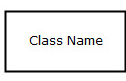
\includegraphics[width=0.2\textwidth]{Figures/table/Sequence/Sequence1}}
		& \setstretch{1.5} {Class แสดงถึงการทำงานของ Use Case ในการส่งหรือรับข้อความ แทนด้วยสัญลักษณ์สี่เหลี่ยมมีชื่อคลาสอยู่ภายใน} \\ \hline
		\raisebox{-\totalheight}{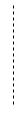
\includegraphics[height=0.1\textheight]{Figures/table/Sequence/Sequence2}}
		& \setstretch{1.5} {Lifeline หรือเส้นอายุขัย แสดงช่วงเวลาตั้งแต่เริ่มสร้าง object ในคลาสนั้น จนกระทั่ง object นั้นถูกทำลาย สัญลักษณ์แทนด้วยเส้นประ} \\ \hline
		\raisebox{-\totalheight}{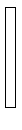
\includegraphics[height=0.1\textheight]{Figures/table/Sequence/Sequence3}}
		& \setstretch{1.5} {Focus of control หรือจุดควบคุม เป็นจุดควบคุมที่ object ใช้ทำการส่งหรือรับข้อความ สัญลักษณ์แทนด้วยสี่เหลี่ยม} \\ \hline
		\raisebox{-\totalheight}{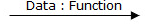
\includegraphics[width=0.3\textwidth]{Figures/table/Sequence/Sequence4}}
		& \setstretch{1.5} {Message คือ ข้อความที่รับส่งระหว่าง Object สัญลักษณ์แทนด้วยลูกศรและประกอบด้วย 2 ส่วน คือ ข้อมูล (Data) และฟังก์ชัน (Function)} \\ \hline
		\raisebox{-\totalheight}{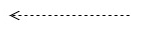
\includegraphics[width=0.3\textwidth]{Figures/table/Sequence/Sequence5}}
		& \setstretch{1.5} {Return Message เป็นข้อมูลที่ส่งกลับหลังจากทำงานเสร็จ} \\ \hline
		\end{tabular}
	\end{table}

	Sequence Diagram ที่ใช้อธิบายการทำงานของแอปพลิเคชันค้นหายาเพื่อคุณซึ่งประกอบไปด้วย 
	การค้นหายาแบบทั่วไป การค้นหายาแบบขั้งสูง การถ่ายรูปเพื่อพิสูจน์เอกลักษณ์ยา และการดูรายละเอียดยา 
	โดยมีรายละเอียดดังต่อไปนี้
	\subsection{Sequence Diagram ของการค้นหายาแบบทั่วไป}

	\begin{figure}[H]
		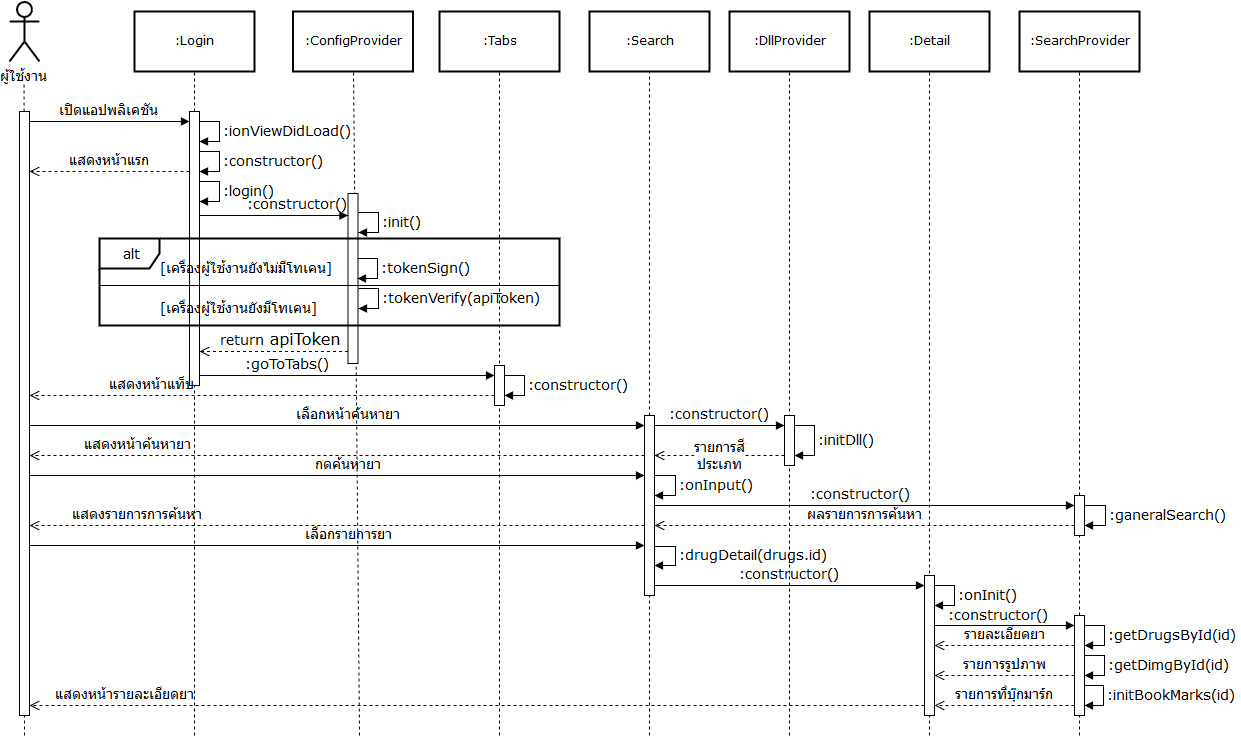
\includegraphics[width=\columnwidth]
		{Figures/3/Sequence-1}
		\caption{Sequence Diagram ของการค้นหายาแบบทั่วไป}
		\label{Fig:Sequence-1}
	\end{figure}

	จากรูปที่ \ref{Fig:Sequence-1} Sequence Diagram ของการค้นหายาแบบทั่วไป 
	สามารถอธิบายได้ดังนี้ 
	เมื่อผู้ใช้งานเปิดแอปพลิเคชันค้นหายาเพื่อคุณ 
	ระบบจะเริ่มต้นการทำที่คลาส Login ด้วยฟังก์ชัน ionViewDidLoad และ constructor 
	เพื่อสร้างหน้าแรกและแสดงหน้าแรกให้ผู้ใช้งาน 
	หลังจากนั้นระบบจะเรียกใช้งานฟังก์ชัน Login 
	และในขณะเดียวกันก็จะเรียกใช้งานคลาส ConfigProvider ฟังก์ชัน Constructor 
	เพื่อเรียกใช้งานฟังก์ชัน init สำหรับกำหนดค่าเริ่มต้นของโทเคน 
	โดยจะมีเงื่อนไขในตรวจสอบเครื่องผู้ใช้งานมีโทเคนหรือไม่ 
	ถ้าหากไม่มีโทเคนจะเรียกใช้งานฟังก์ชัน tokenSign 
	และถ้าหากมีโทเคนจะเรียกใช้งานฟังก์ชัน tokenVerify 
	หลังจากนั้นจะคืน apiToken ที่เป็นผลลัพธ์กลับมาที่คลาส Login 
	และดำเนินการต่อไปด้วยฟังก์ชัน goToTabs 
	สำหรับเรียกใช้งานคลาส Tabs ฟังก์ชัน constructor 
	เพื่อสร้างหน้าแท็บและแสดงหน้าแท็กให้ผู้ใช้งาน 
	จากนั้นเรียกใช้งานคลาส Search ฟังก์ชัน constructor 
	และเรียกใช้งาน DllProvider ฟังก์ชัน initDll 
	เพื่อสร้างหน้าค้นหาและแสดงหน้าค้นหาให้ผู้ใช้งาน 
	เมื่อผู้ใช้งานกดค้นหายาที่หน้าค้นาหายา จะเรียกใช้งานคลาส Search ฟังก์ชัน onInput 
	หลังจากนั้นจะเรียกใช้งานคลาส SearchProvider ฟังก์ชัน constructor 
	และฟังก์ชัน ganeralSearch เพื่อร้องขอการค้นหาไปที่เว็บเซอร์วิสและส่งข้อมูลรายการการค้าหายากลับมายังคลาส Search 
	จากนั้นแสดงที่หน้ารายการค้าหาให้ผู้ใช้งาน 
	เมื่อผู้ใช้งานเลือกรายการยา จะเรียกใช้งานคลาส Search ฟังก์ชัน drugDetail 
	พร้อมกับส่งหมายเลขยาไปกับฟังก์ชัน drugDetail ไปที่คลาส Detail ฟังก์ชัน constructor 
	และฟังก์ชัน onInit เพื่อร้องขอข้อมูลยาจากเว็บเซอร์วิสที่คลาส SearchProvider ผ่านทางฟังก์ชัน getDrugById เพื่อร้องขอข้อมูลรายละเอียดยา และผ่านทางฟังก์ชัน getDimgById 
	เพื่อร้องขอข้อมูลรูปภาพ และฟังก์ชัน initBookMarks เพื่อตรวจสอบรายการที่ถูกบุ๊กมาร์กไว้ 
	และแสดงหน้ารายละเอียดยาแก่ผู้ใช้งาน
	
	\subsection{Sequence Diagram ของการค้นหายาแบบขั้นสูง}

	\begin{figure}[H]
		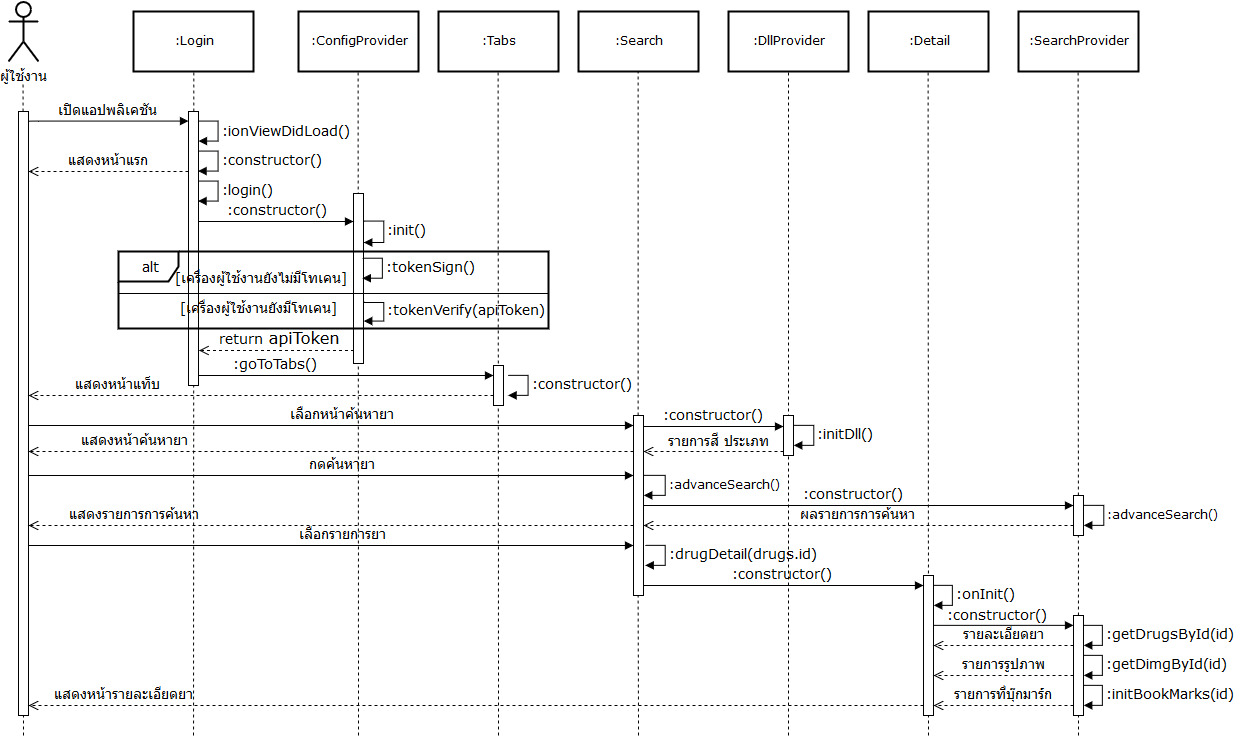
\includegraphics[width=\columnwidth]
		{Figures/3/Sequence-2}
		\caption{Sequence Diagram ของการค้นหายาแบบขั้นสูง}
		\label{Fig:Sequence-2}
	\end{figure}
	
	จากรูปที่ \ref{Fig:Sequence-2} Sequence Diagram ของการค้นหายาแบบขั้นสูง สามารถอธิบายได้ดังนี้ เมื่อผู้ใช้งานเปิดแอปพลิเคชันค้นหายาเพื่อคุณ ระบบจะเริ่มต้นการทำที่คลาส Login ด้วยฟังก์ชัน ionViewDidLoad และ constructor เพื่อสร้างหน้าแรกและแสดงหน้าแรกให้ผู้ใช้งาน หลังจากนั้นระบบจะเรียกใช้งานฟังก์ชัน Login และในขณะเดียวกันก็จะเรียกใช้งานคลาส ConfigProvider ฟังก์ชัน Constructor เพื่อเรียกใช้งานฟังก์ชัน init สำหรับกำหนดค่าเริ่มต้นของโทเคน โดยจะมีเงื่อนไขในตรวจสอบเครื่องผู้ใช้งานมีโทเคนหรือไม่ ถ้าหากไม่มีโทเคนจะเรียกใช้งานฟังก์ชัน tokenSign และถ้าหากมีโทเคนจะเรียกใช้งานฟังก์ชัน tokenVerify หลังจากนั้นจะคืน apiToken ที่เป็นผลลัพธ์กลับมาที่คลาส Login และดำเนินการต่อไปด้วยฟังก์ชัน goToTabs สำหรับเรียกใช้งานคลาส Tabs ฟังก์ชัน constructor เพื่อสร้างหน้าแท็บและแสดงหน้าแท็กให้ผู้ใช้งาน จากนั้นเรียกใช้งานคลาส Search ฟังก์ชัน constructor และเรียกใช้งาน DllProvider ฟังก์ชัน initDll เพื่อสร้างหน้าค้นหาและแสดงหน้าค้นหาให้ผู้งาน เมื่อผู้ใช้งานกดค้นหายา คลาส Search ฟังก์ชัน advanceSearch ในขณะเดียวกันจะเรียกใช้งานคลาส SearchProvider ฟังก์ชัน constructor และฟังก์ชัน advanceSearch เพื่อร้องขอการค้นหาไปที่เว็บเซอร์วิสและส่งข้อมูลรายการการค้าหายากลับมายังคลาส Search จากนั้นแสดงที่หน้ารายการค้าหาให้ผู้ใช้งาน เมื่อผู้ใช้งานเลือกรายการยา จะเรียกใช้งานคลาส Search ฟังก์ชัน drugDetail พร้อมกับส่งหมายเลขยาไปกับฟังก์ชัน ไปที่คลาส Detail ฟังก์ชัน constructor และฟังก์ชัน onInit เพื่อร้องขอข้อมูลยาจากเว็บเซอร์วิสที่คลาส SearchProvider ผ่านทางฟังก์ชัน getDrugById เพื่อร้องขอข้อมูลรายละเอียดยา และผ่านทางฟังก์ชัน getDimgById เพื่อร้องขอข้อมูลรูปภาพ และฟังก์ชัน initBookMarks เพื่อตรวจสอบรายการที่ถูกบุ๊กมาร์กไว้ และแสดงหน้ารายละเอียดยาแก่ผู้ใช้งาน

	\subsection{Sequence Diagram ของการถ่ายรูปภาพเพื่อพิสูจน์เอกลักษณ์ยาเม็ด}	

	\begin{figure}[H]
		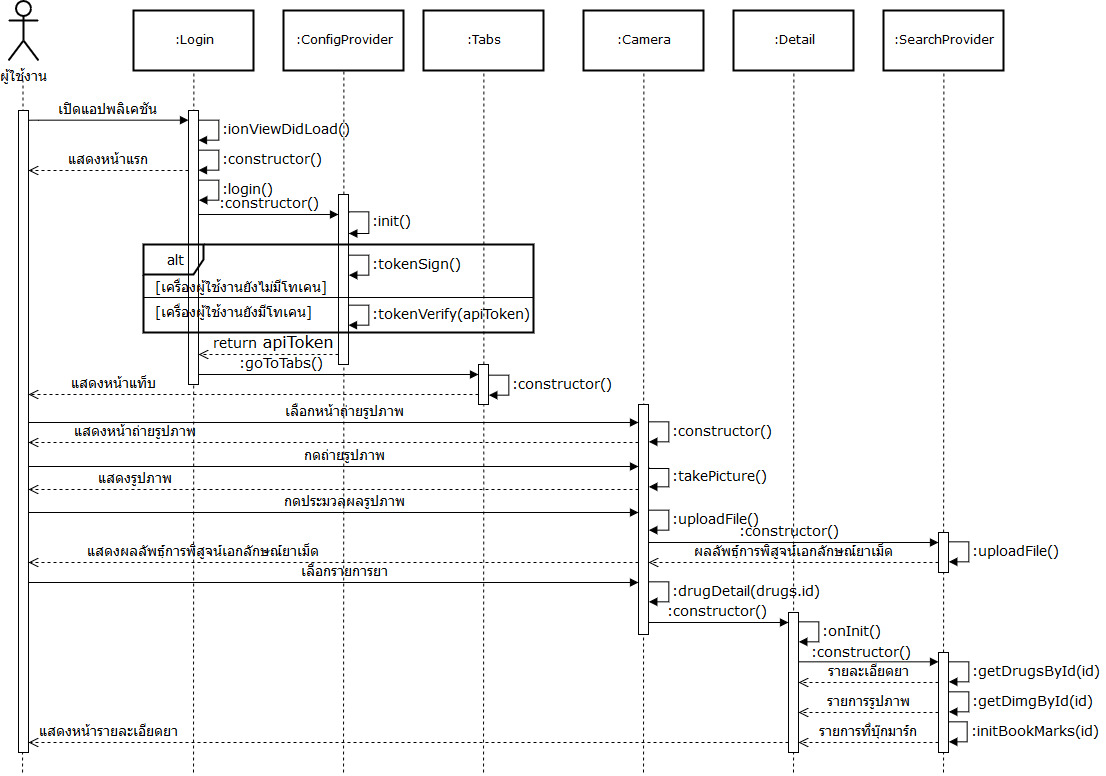
\includegraphics[width=\columnwidth]{Figures/3/Sequence-3}
		\caption{Sequence Diagram ของการถ่ายรูปภาพเพื่อพิสูจน์เอกลักษณ์ยาเม็ด}
		\label{Fig:Sequence-3}
	\end{figure}

	จากรูปที่ \ref{Fig:Sequence-3} Sequence Diagram ของการถ่ายรูปภาพเพื่อพิสูจน์เอกลักษณ์ยาเม็ด สามารถอธิบายได้ดังนี้ เมื่อผู้ใช้งานเปิดแอปพลิเคชันค้นหายาเพื่อคุณ ระบบจะเริ่มต้นการทำที่คลาส Login ด้วยฟังก์ชัน ionViewDidLoad และ constructor เพื่อสร้างหน้าแรกและแสดงหน้าแรกให้ผู้ใช้งาน หลังจากนั้นระบบจะเรียกใช้งานฟังก์ชัน Login และในขณะเดียวกันก็จะเรียกใช้งานคลาส ConfigProvider ฟังก์ชัน Constructor เพื่อเรียกใช้งานฟังก์ชัน init สำหรับกำหนดค่าเริ่มต้นของโทเคน โดยจะมีเงื่อนไขในตรวจสอบเครื่องผู้ใช้งานมีโทเคนหรือไม่ ถ้าหากไม่มีโทเคนจะเรียกใช้งานฟังก์ชัน tokenSign และถ้าหากมีโทเคนจะเรียกใช้งานฟังก์ชัน tokenVerify หลังจากนั้นจะคืน apiToken ที่เป็นผลลัพธ์กลับมาที่คลาส Login และดำเนินการต่อไปด้วยฟังก์ชัน goToTabs สำหรับเรียกใช้งานคลาส Tabs ฟังก์ชัน constructor เพื่อสร้างหน้าแท็บและแสดงหน้าแท็กให้ผู้ใช้งาน จากนั้นเรียกใช้งานคลาส Camera ฟังก์ชัน constructor เพื่อสร้างหน้าการถ่ายรูปเพื่อพิสูจน์เอกลักษณ์ยา เมื่อผู้ใช้งานกดถ่ายรูปภาพยาจะเรียกใช้งานฟังก์ชัน takePicture และจะแสดงรูปรูปที่ถ่ายได้ให้ผู้ใช้งาน เมื่อผู้ใช้งานกดประมวลผลภาพจะเรียกใช้งานฟังก์ชัน uploadFile ในขณะเดียวกันจะเรียกใช้งานคลาส SearchProvider ฟังก์ชัน constructor และฟังก์ชัน uploadFile เพื่อร้องขอไปประมวลผลภาพที่เว็บเซอร์วิสและส่งผลลัพธ์กลับมาที่คลาส Camera เพื่อแสดงผลลัพธ์การพิสูจน์เอกลักษณ์ยาให้ผู้ใช้งาน เมื่อผู้ใช้งานเลือกรายการยา จะเรียกใช้งานคลาส Search ฟังก์ชัน drugDetail พร้อมกับส่งหมายเลขยาไปกับฟังก์ชัน ไปที่คลาส Detail ฟังก์ชัน constructor และฟังก์ชัน onInit เพื่อร้องขอข้อมูลยาจากเว็บเซอร์วิสที่คลาส SearchProvider ผ่านทางฟังก์ชัน getDrugById เพื่อร้องขอข้อมูลรายละเอียดยา และผ่านทางฟังก์ชัน getDimgById เพื่อร้องขอข้อมูลรูปภาพ และฟังก์ชัน initBookMarks เพื่อตรวจสอบรายการที่ถูกบุ๊กมาร์กไว้ และแสดงหน้ารายละเอียดยาแก่ผู้ใช้งาน
	
	\subsection{Sequence Diagram ของการดูรายการบุ๊กมาร์ก}

	\begin{figure}[H]
		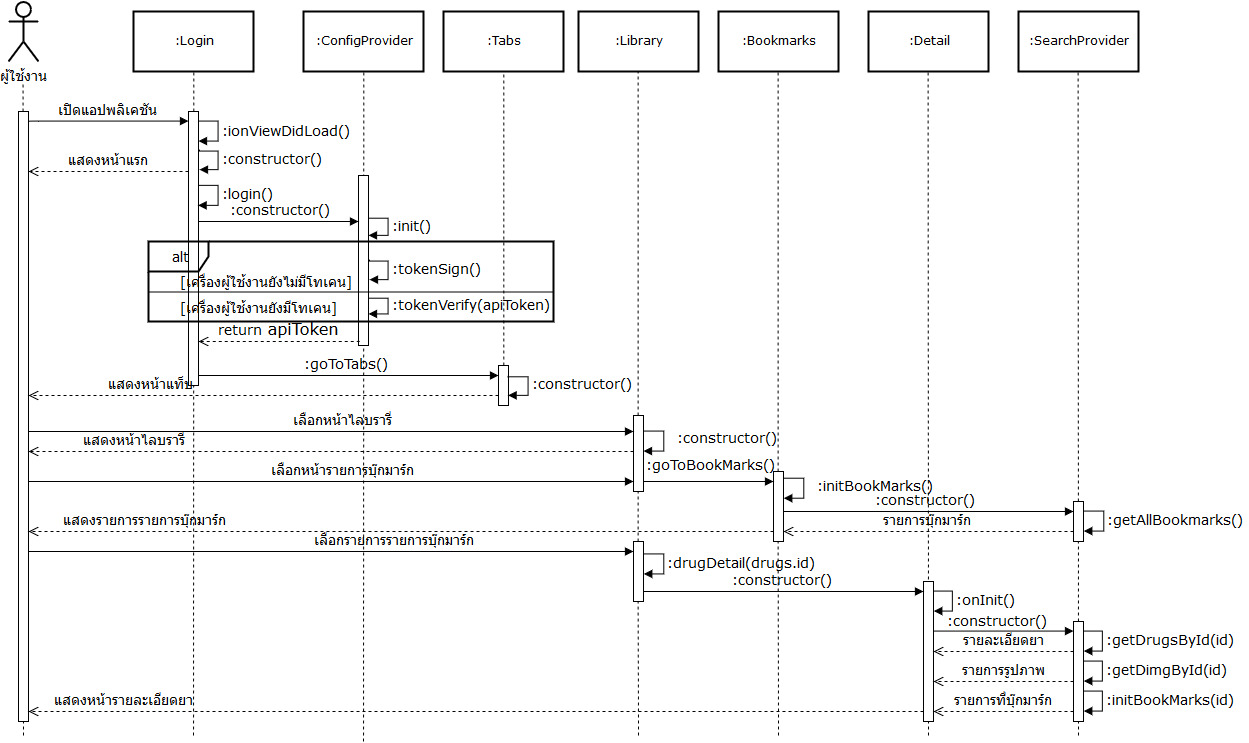
\includegraphics[width=\columnwidth]
		{Figures/3/Sequence-4}
		\caption{Sequence Diagram ของการดูรายการบุ๊กมาร์ก}
		\label{Fig:Sequence-4}
	\end{figure}

	จากรูปที่ \ref{Fig:Sequence-4} Sequence Diagram ของการดูรายละเอียดยา สามารถอธิบายได้ดังนี้ เมื่อผู้ใช้งานเปิดแอปพลิเคชันค้นหายาเพื่อคุณ ระบบจะเริ่มต้นการทำที่คลาส Login ด้วยฟังก์ชัน ionViewDidLoad และ constructor เพื่อสร้างหน้าแรกและแสดงหน้าแรกให้ผู้ใช้งาน หลังจากนั้นระบบจะเรียกใช้งานฟังก์ชัน Login และในขณะเดียวกันก็จะเรียกใช้งานคลาส ConfigProvider ฟังก์ชัน Constructor เพื่อเรียกใช้งานฟังก์ชัน init สำหรับกำหนดค่าเริ่มต้นของโทเคน โดยจะมีเงื่อนไขในตรวจสอบเครื่องผู้ใช้งานมีโทเคนหรือไม่ ถ้าหากไม่มีโทเคนจะเรียกใช้งานฟังก์ชัน tokenSign และถ้าหากมีโทเคนจะเรียกใช้งานฟังก์ชัน tokenVerify หลังจากนั้นจะคืน apiToken ที่เป็นผลลัพธ์กลับมาที่คลาส Login และดำเนินการต่อไปด้วยฟังก์ชัน goToTabs สำหรับเรียกใช้งานคลาส Tabs ฟังก์ชัน constructor เพื่อสร้างหน้าแท็บและแสดงหน้าแท็กให้ผู้ใช้งาน เมื่อผู้ใช้งานเลือกหน้าไลบรารี่ จะเรียกใช้งานคลาส Library ฟังก์ชัน goToBookMarks เพื่อเรียกใช้งานคลาส Bookmarks ฟังก์ชัน initBookMarks ในขณะเดียวกันจะเรียกใช้งานคลาส SearchProvider ฟังก์ชัน constructor และฟังก์ชัน getAllBookmarks เพื่อดึงรายการบุ๊กมาร์กจากเครื่องผู้ใช้งานมา จากนั้นจะแสดงหน้ารายการบุ๊กมาร์กให้ผู้ใช้งาน เมื่อผู้ใช้งานเลือกรายการยา จะเรียกใช้งานคลาส Search ฟังก์ชัน drugDetail พร้อมกับส่งหมายเลขยาไปกับฟังก์ชัน ไปที่คลาส Detail ฟังก์ชัน constructor และฟังก์ชัน onInit เพื่อร้องขอข้อมูลยาจากเว็บเซอร์วิสที่คลาส SearchProvider ผ่านทางฟังก์ชัน getDrugById เพื่อร้องขอข้อมูลรายละเอียดยา และผ่านทางฟังก์ชัน getDimgById เพื่อร้องขอข้อมูลรูปภาพ และฟังก์ชัน initBookMarks เพื่อตรวจสอบรายการที่ถูกบุ๊กมาร์กไว้ และแสดงหน้ารายละเอียดยาแก่ผู้ใช้งาน


\newpage
\section{State Diagram}
	State Diagram เป็นภาพแผนที่แสดงอ็อบเจ็กต์แต่ละตัว โดยสถานะรวมของระบบเกิดจากสถานะย่อยของอ็อบเจ็กต์แต่ละตัวรวมกันเป็นกลไกที่ทำให้ระบบมีการเปลี่ยนสถานะคือการส่ง message ในทาง Object orientation คือการเรียกใช้ฟังก์ชันของอ็อบเจ็กต์นั้นเอง ซึ่งส่วนประกอบและสัญลักษณ์ที่ใช้ในการเขียน State Diagram แสดงในตารางที่ \ref{tab:state}
	
	\begin{table}[H]
		\centering
		\caption{สัญลักษณ์ของ State Diagram}
		\label{tab:state}
		\begin{tabular}{| c	| p{10cm} |}
		\hline
		\textbf{สัญลักษณ์} & \multicolumn{1}{c|}{\textbf{การใช้งาน}} \\ \hline
		\raisebox{-\totalheight}{
\includegraphics[width=8mm]{Figures/table/state/state1}}
		& \setstretch{1.5} {Initial state คือสถานะเริ่มต้นแสดงถึงอ็อบเจ็กต์ที่เกิดขึ้น} \\ \hline
		\raisebox{-\totalheight}{
\includegraphics[width=0.1\textwidth]{Figures/table/state/state2}}
		& \setstretch{1.5} {Initial state คือสถานะเริ่มต้นแสดงถึงอ็อบเจ็กต์ที่เกิดขึ้น} \\ \hline
		\raisebox{-\totalheight}{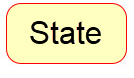
\includegraphics[width=0.2\textwidth]{Figures/table/state/state3}}
		& \setstretch{1.5} {State คือแสดงสถานะอ็อบเจ็กต์} \\ \hline
		\raisebox{-\totalheight}{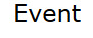
\includegraphics[width=0.2\textwidth]{Figures/table/state/state4}}
		& \setstretch{1.5} {Event คือเหตุการณ์ที่เกิดขึ้นทำให้เกิดการเปลี่ยนสถานะ โดยมีเงื่อนไข ซึ่งอ็อบเจ็กต์จะเปลี่ยนสถานะเมื่อเงื่อนไขดังกว่างเป็นจริง} \\ \hline
		\raisebox{-\totalheight}{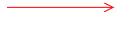
\includegraphics[width=0.3\textwidth]{Figures/table/state/state5}}
		& \setstretch{1.5} {Transition คือการเปลี่ยนสถานะแสดงถึงการเปลี่ยนสถานะของอ็อบเจ็กต์จากสถานะหนึ่งไปยังสถานะอื่น} \\ \hline
		\end{tabular}
	\end{table}


	State Diagram ใช้สำหรับอธิบายการทำงานของแอปพลิเคชันค้นหายาเพื่อคุณซึ่งประกอบไปด้วย ส่วนการค้นหายาและการแสดงรายละเอียดยา และส่วนการถ่ายรูปเพื่อการพิสูจน์เอกลักษณ์ยา โดยมีรายละเอียดดังต่อไปนี้

	\begin{figure}[H]
		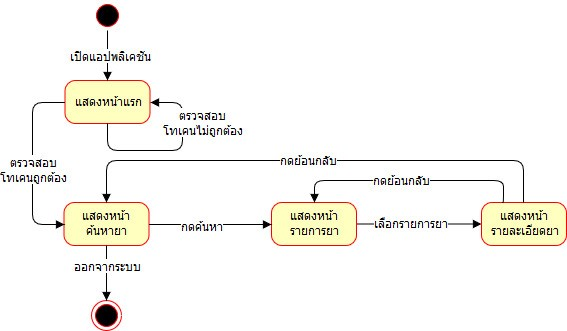
\includegraphics[width=\columnwidth]{Figures/3/state1}
		\caption{State Diagram ส่วนการค้นหายาและการแสดงรายละเอียดยา}
		\label{Fig:state1}
	\end{figure}

	จากรูปที่ \ref{Fig:state1} เป็น State Diagram ของส่วนการค้นหายาและการแสดงรายละเอียดยา สามารถอธิบายได้ดังต่อไปนี้ ผู้ใช้งานเปิดแอปพลิเคชันขึ้นมาระบบจะอยู่ในสถานะแสดงหน้าแรก เมื่อระบบตรวจสอบความถูกต้องของโทเคนสำเร็จ ระบบจะอยู่ในสถานะแสดงค้นหายา เมื่อผู้ใช้งานกดค้นหายาระบบจะอยู่ในสถานะแสดงหน้ารายการยา เมื่อผู้ใช้งานเลือกรายการยาเพื่อย้ายสถานะของระบบไปที่สถานะแสดงหน้ารายะเอียดยา จากนั้นผู้ใช้งานสามารถกดย้อนกลับ (รายการยา) เพื่อย้ายสถานะของระบบไปที่สถานะแสดงหน้ารายการยาและผู้ใช้งานสามารถกดย้อมกลับ (ค้นหายา) เพื่อย้ายสถานะของระบบไปที่สถานะแสดงหน้าค้นหา

	\begin{figure}[H]
		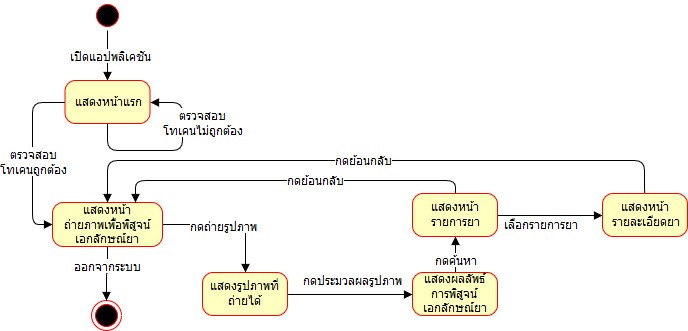
\includegraphics[width=\columnwidth]{Figures/3/state2}
		\caption{State Diagram ส่วนการถ่ายรูปเพื่อการพิสูจน์เอกลักษณ์ยา}
		\label{Fig:state2}
	\end{figure}

	จากรูปที่ \ref{Fig:state2} เป็น State Diagram ของส่วนการถ่ายรูปเพื่อการพิสูจน์เอกลักษณ์ยา สามารถอธิบายรายละเอียดได้ดังต่อไปนี้ ผู้ใช้งานเปิดแอปพลิเคชันค้นหายาเพื่อคุณขึ้นมาระบบจะอยู่ในสถานะแสดงหน้าแรก เมื่อระบบตรวจสอบความถูกต้องของโทเคนสำเร็จ สถานะของระบบจะถูกย้ายไปที่สถานะแสดงหน้าถ่ายภาพเพื่อพิสูจน์เอกลักษณ์ยา เมื่อผู้ใช้งานกดถ่ายรูปภาพสถานะของระบบจะย้ายไปที่สถานะแสดงรูปภาพที่ถ่ายได้ เมื่อผู้ใช้งานกดประมวลผลรูปภาพระบบจะย้ายไปที่สถานะแสดงผลลัพธ์การพิสูจน์เอกลักษณ์ยา เมื่อผู้ใช้งานกดค้นหายาสถานะของระบบจะย้ายไปที่สถานะหน้ารายการยา ผู้ใช้งานสามารถกดย้อนกลับเพื่อย้ายสถานะระบบไปที่สถานะแสดงหน้าถ่ายภาพเพื่อพิสูจน์เอกลักษณ์ยาและผู้ใช้งานสามารถเลือกรายการยาเพื่อย้ายสถานะระบบไปที่สถานะแสดงหน้ารายละเอียดยา และเมื่อผู้ใช้กดย้อมกลับเพื่อย้ายสถานะระบบไปที่สถานะแสดงหน้าถ่ายภาพเพื่อพิสูจน์เอกลักษณ์ยา
\newpage
\section{การประมวลผลภาพยาเม็ดเพื่อการพิสูจน์เอกลักษณ์ยาเม็ด}
	ส่วนการประมวลผลภาพยาเม็ดเพื่อการพิสูจน์เอกลักษณ์ยาเม็ดพัฒนาด้วยภาษา Javascript มีรายละเอียดดังต่อไปนี้

	\begin{itemize}
		\item ทดลองการจำแนกรูปทรงของยาเม็ดด้วยการเรียนรู้ของเครื่อง (Machines Learning)
		\item การหาขนาดด้านยาวของเม็ดยาโดยใช้วัถตุอ้างอิงที่รู้ขนาด
		\item การหาลักษณะสีของยาเม็ด
	\end{itemize}

	\subsection{ทดลองการจำแนกรูปทรงของยาเม็ดด้วยการเรียนรู้ของเครื่อง (Machines Learning)}
		การจำแนกรูปทรงด้วยการเรียนรู้ของเครื่องโดยใช้อัลกอริทึมทั้งหมด 3 อัลกอริทึม ได้แก่ Support Vector Machines (SVM), K-nearest neighbor (KNN) และ Random Forest Classifier (RFC) เพื่อหาความถูกต้องที่มากที่สุดของแบบจำลองที่นำมาใช้งานจริง และข้อมูลรูปทรงเม็ดยาที่ใช้ในการเตรียมการฝึกและทดสอบแบบจำลองทั้งสามแบบจำลองเป็นข้อมูลชุดเดียวกัน 
		\begin{enumerate}
			\item การเตรียมข้อมูล
			

			รูปทรงเม็ดยามีทั้งหมด 8 รูปทรง มีสี่เหลี่ยม สามเหลี่ยม วงกลม วงวี แคปซูล หัวท้ายมน หกเหลี่ยมและแปดเหลี่ยม 
			แต่เนื่องจากรูปทรงวงรี แคปซูลและหัวท้ายมน มีรูปทรงที่คล้ายกันจึงได้รวมรูปทรงทั้งสามรูปทรงเข้าด้วยกัน 
			เป็นรูปทรงแคปซูล ดังนั้นรูปทรงเม็ดยาที่ใช้ในการฝึกและทดสอบแบบจำลองจะมีทั้งหมด 6 รูปทรง 
			คือ 
			รูปทรงสี่เหลี่ยม จำนวนรูปภาพที่ใช้สำหรับฝึกทั้งหมด 44 รูปภาพ และจำนวนรูปภาพที่ใช้สำหรับทดสอบ 20 รูปภาพ
			รูปทรงสามเหลี่ยม จำนวนรูปภาพที่ใช้สำหรับฝึกทั้งหมด 45 รูปภาพ และจำนวนรูปภาพที่ใช้สำหรับทดสอบ 20 รูปภาพ
			รูปทรงวงกลม จำนวนรูปภาพที่ใช้สำหรับฝึกทั้งหมด 29 รูปภาพ และจำนวนรูปภาพที่ใช้สำหรับทดสอบ 20 รูปภาพ
			รูปทรงแคปซูลจำนวนรูปภาพที่ใช้สำหรับฝึกทั้งหมด 38 รูปภาพ และจำนวนรูปภาพที่ใช้สำหรับทดสอบ 20 รูปภาพ
			รูปทรงหกเหลี่ยม จำนวนรูปภาพที่ใช้สำหรับฝึกทั้งหมด 59 รูปภาพ และจำนวนรูปภาพที่ใช้สำหรับทดสอบ 20 รูปภาพ
			และรูปทรงแปดเหลี่ยม จำนวนรูปภาพที่ใช้สำหรับฝึกทั้งหมด 43 รูปภาพ และจำนวนรูปภาพที่ใช้สำหรับทดสอบ 20 รูปภาพ
			มีรายละเอียดแสดงดังตารางที่ \ref{tab:data-set} 

			\begin{table}[H]
				\centering
				\caption{ตารางแสดงจำนวนของข้อมูลรูปทรงยาเม็ดที่ใช้ฝึกและทดสอบ}
				\label{tab:data-set}
				\begin{tabular}{ | c | c | c | }
				\hline
				\textbf{รูปทรง}} &
				\textbf{จำนวนรูปที่ใช้ฝึก} &
				\textbf{จำนวนรูปที่ใช้ทดสอบ} \\ \hline
				สี่เหลี่ยม   & 
				44  &  
				20  \\ \hline
				สามเหลี่ยม & 
				45 &  
				20  \\ \hline
				วงกลม    & 
				29  & 
				20  \\ \hline
				แคปซูล   &  
				38 &  
				20 \\ \hline
				หกเหลี่ยม  & 
				59  & 
				20   \\ \hline
				แปดเหลี่ยม & 
				43  &  
				20  \\ \hline
				\end{tabular}
			\end{table}
			

			\begin{figure}[H]
				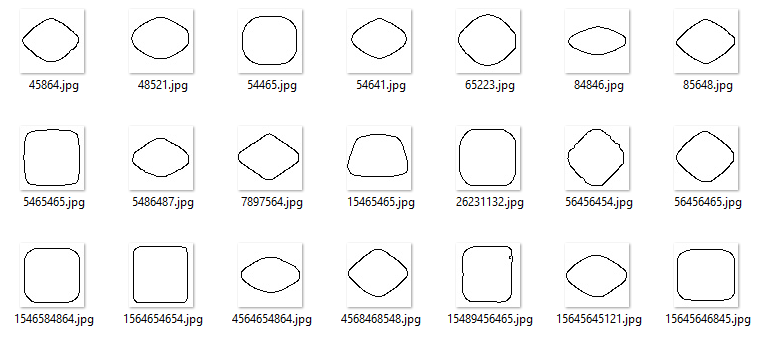
\includegraphics[width=\columnwidth]{Figures/3/opencv1}
				\caption{ตัวอย่างข้อมูลสำหรับการฝึกแบบจำลองรูปทรงสี่เหลี่ยม}
				\label{Fig:opencv1}
			\end{figure}

			\begin{figure}[H]
				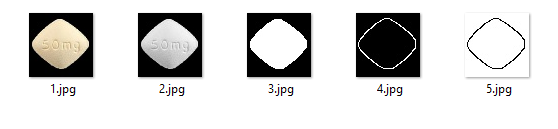
\includegraphics[width=\columnwidth]{Figures/3/opencv2}
				\caption{แสดงการขั้นตอนการทำความสะอาดข้อมูลรูปสำหรับใช้ฝึกและสอน}
				\label{Fig:opencv2}
			\end{figure}
			จากรูปที่ \ref{Fig:opencv1} รูปภาพตัวอย่างข้อมูลสำหรับการฝึกแบบจำลองรูปทรงสี่เหลี่ยม 
			รูปทรงของยารูปทรงสี่เหลี่ยมมีหลายรูปแบบ 
			ได้แก่
			รูปทรงสี่เหลี่ยมขนมเปียกปูน
			รูปทรงสี่เหลี่ยมจัตุรัส
			รูปทรงสี่เหลี่ยมผืนผ้า 
			และรูปทรงสี่เหลี่ยมขนมเปียกปูน จากรูปทรงทั้งหมด คือ รูปทรงสี่เหลี่ยม
			จากรูปที่ \ref{Fig:opencv2} แสดงลำดับการทำความสะอาดข้อมูลรูปภาพก่อนจะใช้ฝึกและสอนรูปแบบจำลอง SVM kNN และ RFC โดยรูปที่ 1.jpg คือรูปภาพต้นฉบับขนาด 64x64 พิกเซล รูปที่ 2.jpg คือรูปภาพสีเทาที่ถูกเป็นแปลงจาก BGR รูปที่ 3.jpg คือรูปที่ถูกปรับ Threshold รูปที่ 4.jpg คือรูปที่ผ่านการตรวจหา Canny Edge และรูปภาพสุดท้ายรูปที่ 5.jpg คือรูปที่ผ่านการสลับบิท ตามลำดับ

			\item การฝึกและทดสอบแบบจำลอง


			การกำหนดค่าพารามิเตอร์ของแบบจำลอง SVM คือ กำหนดชนิดของ kernelType เป็น RBF กำหนดค่า c เป็น 12.5 และ กำหนดค่า gamma เป็น 0.50625
			แสดงดังรูปที่ \ref{Fig:svm-para} 
						
			\begin{figure}[H]
				{\setstretch{1.0}\begin{lstlisting}
const svm = new cv.SVM({
	kernelType: cv.ml.SVM.RBF,
	c: 12.5,
	gamma: 0.50625
});
				\end{lstlisting}}
				\caption{การกำหนดค่าพารามิเตอร์ของแบบจำลอง SVM}
				\label{Fig:svm-para}
			\end{figure}
			
			จากตารางที่ \ref{tab:SVM} 
			จะเห็นได้ว่ารูปทรงที่ใช้ฝึกและทดสอบมี 6 รูปทรง 
			รูปทรงสี่เหลี่ยมจำแนกถูกต้อง 20 รูปภาพ คิดเป็นร้อยละ 100 
			รูปทรงสามเหลี่ยมจำแนกถูกต้อง 19 รูปภาพ คิดเป็นร้อยละ 95 
			รูปทรงวงกลมจำแนกถูกต้อง 19 รูปภาพ คิดเป็นร้อยละ 95 
			รูปทรงแคปซูลจำแนกถูกต้อง 20 รูปภาพ คิดเป็นร้อยละ 100 
			รูปทรงหกเหลี่ยมจำแนกถูกต้อง 18 รูปภาพ คิดเป็นร้อยละ 90 
			รูปทรงแปดเหลี่ยมจำแนกถูกต้อง 17 รูปภาพ คิดเป็นร้อยละ 85 
			
			ดังนั้นการฝึกและทดสอบแบบจำลอง SVM มีความถูกต้องโดยเฉลี่ยร้อยละ 94.17

			% \begin{table}[H]
			% 	\caption{แสดงความถูกต้องของแบบจำลอง SVM}
			% 	\label{tab:SVM}				
			% 	\begin{tabular}{c}
			% 		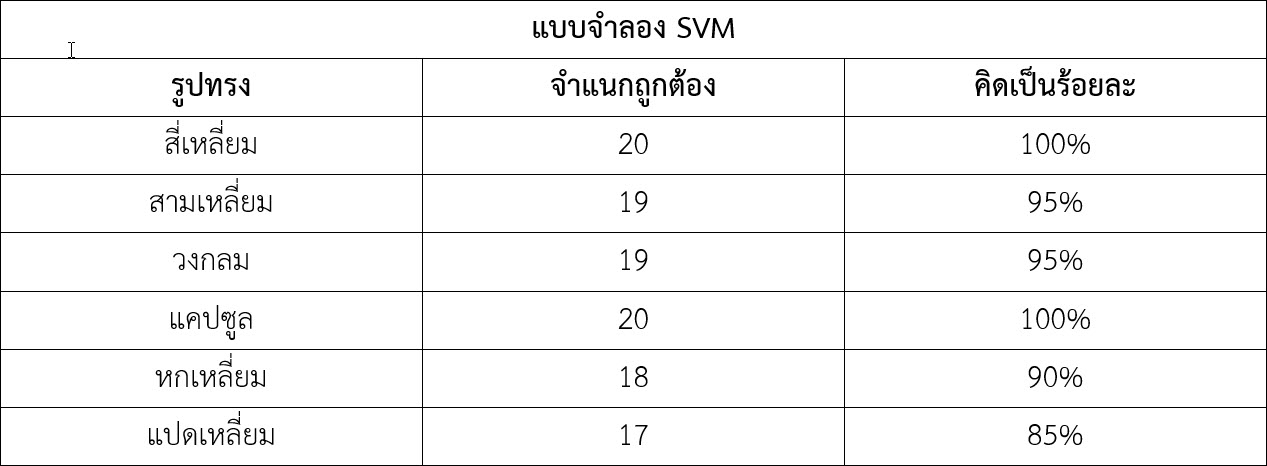
\includegraphics[width=\columnwidth]{Figures/table/SVM}	\\ 
			% 	\end{tabular}
			% \end{table}
			\begin{table}[H]
				\centering
				\caption{แสดงความถูกต้องของแบบจำลอง SVM}
				\label{tab:SVM}
				\begin{tabular}{|p{4cm}|p{4cm}|p{4cm}|}
				\hline
				\multicolumn{1}{|c}{\textbf{รูปทรง}} &
				\multicolumn{1}{|c}{\textbf{จำแนกถูกต้อง}} &
				\multicolumn{1}{|c|}{\textbf{คิดเป็นร้อยละ}} \\ \hline
				\multicolumn{1}{|c}{\textbf{สี่เหลี่ยม}}   & 
				\multicolumn{1}{|c}{\textbf{20}}  &  
				\multicolumn{1}{|c|}{\textbf{100\%}}  \\ \hline
				\multicolumn{1}{|c}{\textbf{สามเหลี่ยม}} & 
				\multicolumn{1}{|c}{\textbf{19}}  &  
				\multicolumn{1}{|c|}{\textbf{95\%}}  \\ \hline
				\multicolumn{1}{|c}{\textbf{วงกลม}}    & 
				\multicolumn{1}{|c}{\textbf{19}}  & 
				\multicolumn{1}{|c|}{\textbf{95\%}}  \\ \hline
				\multicolumn{1}{|c}{\textbf{แคปซูล}}   &  
				\multicolumn{1}{|c}{\textbf{20}} &  
				\multicolumn{1}{|c|}{\textbf{100\%}} \\ \hline
				\multicolumn{1}{|c}{\textbf{หกเหลี่ยม}}  & 
				\multicolumn{1}{|c}{\textbf{18}}  & 
				\multicolumn{1}{|c|}{\textbf{90\%}}   \\ \hline
				\multicolumn{1}{|c}{\textbf{แปดเหลี่ยม}} & 
				\multicolumn{1}{|c}{\textbf{17}}  &  
				\multicolumn{1}{|c|}{\textbf{85\%}}  \\ \hline
				\end{tabular}
			\end{table}
			
			การกำหนดค่าพารามิเตอร์ของแบบจำลอง KNN ดังนี้ 
			train คือ ชุดข้อมูลสำหรับการใช้ฝึกสอนแบบจำลอง 
			cv2.ml.ROW{\_}SAMPLE คือ การกำหนดรูปแบบของชุดข้อมูลเป็นแบบแถว 
			train{\_}labels คือ คลาสของชุดข้อมูลสำหรับการใช้ฝึกสอนแบบจำลอง 
			และ k คือ จำนวนของคลาสที่ใกล้เคียงสูงสุด
			แสดงดังรูปที่  \ref{Fig:knn-para}

			\begin{figure}[H]
				{\setstretch{1.0}\begin{lstlisting}
knn = cv2.ml.KNearest_create()
knn.train(train, cv2.ml.ROW_SAMPLE, train_labels)
result = knn.findNearest(test, k=6)
				\end{lstlisting}}
				\caption{การกำหนดค่าพารามิเตอร์ของแบบจำลอง KNN}
				\label{Fig:knn-para}
			\end{figure}

			จากตารางที่ \ref{tab:KNN}	 การฝึกและทดสอบแบบจำลอง kNN โดยจะเริ่มจากค่า 
			k = 1 ถึง k = 6 จะเห็นได้ว่า 
			K ที่ 1 มีค่าความถูกต้องของแบบจำลองร้อยละ 79.17 
			K ที่ 2 มีค่าความถูกต้องของแบบจำลองร้อยละ 76.67 
			K ที่ 3 มีค่าความถูกต้องของแบบจำลองร้อยละ 74.17 
			K ที่ 4 มีค่าความถูกต้องของแบบจำลองร้อยละ 70.83 
			K ที่ 5 มีค่าความถูกต้องของแบบจำลองร้อยละ 72.50 
			และ K ที่ 6 มีค่าความถูกต้องของแบบจำลองร้อยละ 71.67 

			ดังนั้นการฝึกและทดสอบแบบจำลอง kNN มีความถูกต้องโดยเฉลี่ยร้อยละ 74.17 
			และ K ที่ 1 มีค่าความถูกต้องสูงที่สุดของแบบจำลองร้อยละ 79.17

			% \begin{table}[H]
			% 	\caption{แสดงความถูกต้องของแบบจำลอง kNN}
			% 	\label{tab:KNN}				
			% 	\begin{tabular}{c}
			% 		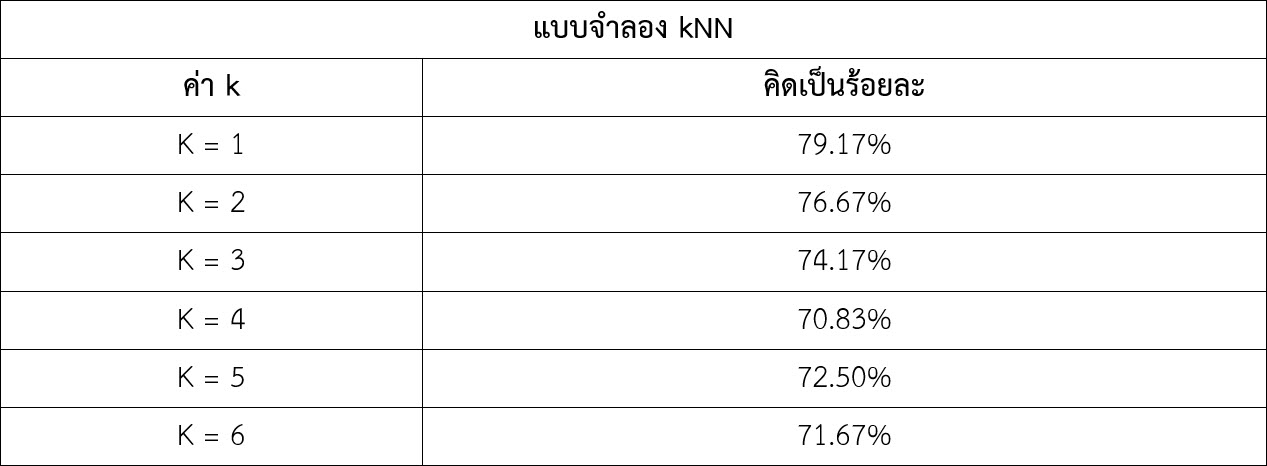
\includegraphics[width=\columnwidth]{Figures/table/KNN}	\\ 
			% 	\end{tabular}
			% \end{table}
			\begin{table}[H]
				\centering
				\caption{แสดงความถูกต้องของแบบจำลอง kNN}
				\label{tab:KNN}
				\begin{tabular}{|c|c|}
				\hline
				ค่า k & คิดเป็นร้อยละ \\ \hline				
				K = 1 &  79.17\% \\ \hline
				K = 2 &  76.67\% \\ \hline
				K = 3 &  74.17\% \\ \hline
				K = 4 &  70.83\% \\ \hline
				K = 5 &  72.50\% \\ \hline
				K = 6 &  71.67\% \\ \hline
				\end{tabular}
			\end{table}

			การกำหนดค่าพารามิเตอร์ของแบบจำลอง KNN 
			โดยการกำหนดพารามิเตอร์ n{\_}estimators คือ จำนวนของต้นไม้ตัดสินใจในการสร้างแบบจำลอง 
			train คือ ชุดข้อมูลสำหรับการใช้ฝึกสอนแบบจำลอง 
			และ train{\_}labels คือ คลาสของชุดข้อมูลสำหรับการใช้ฝึกสอนแบบจำลอง 
			แสดงดังรูปที่ \ref{Fig:rfc-para}

			\begin{figure}[H]
				{\setstretch{1.0}\begin{lstlisting}
RFC = RandomForestClassifier(n_estimators=100)
RFC.fit(train, train_labels)
				\end{lstlisting}}
				\caption{การกำหนดค่าพารามิเตอร์ของแบบจำลอง RFC}
				\label{Fig:rfc-para}
			\end{figure}

			จากตารางที่ \ref{tab:RFC} การฝึกและทดสอบแบบจำลอง RFC 
			โดยมีการปรับค่า {N\_estimators} ตั้งแต่ 10 ถึง 100 
			จะเห็นได้ว่า {N\_estimators} เท่ากับ 10 มีค่าความถูกต้องของแบบจำลองร้อยละ 53.33 
			{N\_estimators} เท่ากับ 30 มีค่าความถูกต้องของแบบจำลองร้อยละ 67.50 
			{N\_estimators} เท่ากับ 50 มีค่าความถูกต้องของแบบจำลองร้อยละ 66.67 
			{N\_estimators} เท่ากับ 70 มีค่าความถูกต้องของแบบจำลองร้อยละ 65.00 
			{N\_estimators} เท่ากับ 90 มีค่าความถูกต้องของแบบจำลองร้อยละ 69.17 
			และ {N\_estimators} เท่ากับ 100 มีค่าความถูกต้องของแบบจำลองร้อยละ 66.67

			ดังนั้นการฝึกและทดสอบแบบจำลอง RFC มีความถูกต้องโดยเฉลี่ยร้อยละ 64.72 และ {N\_estimators} เท่ากับ 90 มีค่าความถูกต้องสูงที่สุดของแบบจำลองร้อยละ 69.17 

			% \begin{table}[H]
			% 	\caption{แสดงความถูกต้องของแบบจำลอง RFC}
			% 	\label{tab:RFC}				
			% 	\begin{tabular}{c}
			% 		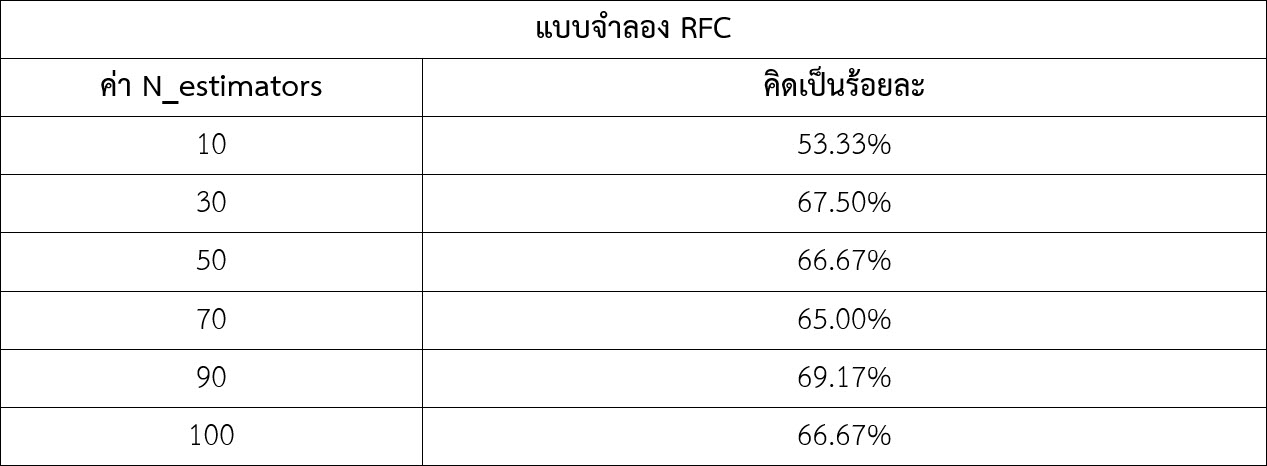
\includegraphics[width=\columnwidth]{Figures/table/RFC}	\\ 
			% 	\end{tabular}
			% \end{table}
			\begin{table}[H]
				\centering
				\caption{แสดงความถูกต้องของแบบจำลอง RFC}
				\label{tab:RFC}
				\begin{tabular}{|c|c|}
				\hline
				ค่า N\_estimators & คิดเป็นร้อยละ \\ \hline				
				10 &  53.33\% \\ \hline
				30 &  67.50\% \\ \hline
				50 &  66.67\% \\ \hline
				70 &  65.00\% \\ \hline
				90 &  69.17\% \\ \hline
				100 &  66.67\% \\ \hline
				\end{tabular}
			\end{table}



			\item สรุปผลการทำลอง
			
			
			จากตารางที่ \ref{tab:SVM} \ref{tab:KNN} และ \ref{tab:RFC} 
			จะเห็นได้ว่าแบบจำลอง SVM มีค่าความถูกต้องร้อยละ 94.17 
			ซึ่งมีค่าความถูกต้องมากกว่าแบบจำลอง 
			kNN มีค่าความถูกต้องร้อยละ 79.17
			และแบบจำลอง RFC มีค่าความถูกต้องร้อยละ 69.17 ตามลำดับ 
			
			ดังนั้นผู้พัฒนาจึงเลือกใช้แบบจำลอง SVM 
			ที่มีความถูกต้องในการจำแนกรูปทรงเม็ดยาสูงที่สุด 
			และนำมาใช้เป็นแบบจำลองในโครงงานแอปพลิเคชันค้นหายาเพื่อคุณ

			\begin{table}[H]
				\centering
				\caption{สรุปผลการทดลอง}
				\label{tab:summary}
				\begin{tabular}{| p{5cm}|c|}
				\hline
				\multicolumn{1}{|c|}{\textbf{แบบจำลอง}} & ค่าความถูกต้อง \\ \hline				
				Support vector machines &  94.17\% \\ \hline
				k-Nearest Neighbors &  79.17\% \\ \hline
				Random Forest Classifier &  69.17 \% \\ \hline
				\end{tabular}
			\end{table}

		\end{enumerate}

	\subsection{การหาขนาดด้านยาวของเม็ดยาโดยใช้วัถตุอ้างอิงที่รู้ขนาด}
		การถ่ายรูปภาพเพื่อหาขนาดด้านยาวของเม็ดยาจำเป็นต้องใช้วัถตุอ้างอิงสีดำที่มีขนาดเท่ากับ 11.3 x 7.3 เซนติเมตร หรือเท่ากับการใช้กระดาษ A4 พับครึ่ง 3 ครั้ง จากรูปที่ \ref{Fig:opencv3}2 พื้นที่สีดำคือวัตถุอ้างอิงที่ทราบขนาด และกรอบสีเหลืองคือ Contour ที่ตรวจพบ หน่วยในภาพเป็นหน่วยพิกเซล ดังนั้นสามารถใช้การเทียบบัญญัติไตรยางศ์เพื่อหาขนาดด้านยาวได้ “1 พิกเซล เท่ากับกี่เซนติเมตร”
	
		ถ้าสมมติให้ขนาดของวัถตุอ้างอิงเท่ากับ 146.9 x 94.9 พิกเซล และกรอบสีเหลืองมีขนาดเท่ากับ 40 x 23 พิกเซล และวัถตุอ้างอิงขนาดเท่ากับ 11.3 x 7.3 เซนติเมตร เมื่อ 146.9 พิกเซล เท่ากับ 11.3 เซนติเมตร และ 1 พิกเซล เท่ากับ ( 11.3 / 146.9 ) = 0.0769 เซนติเมตร ดังนั้น 40 พิกเซล เท่ากับ ( 40 x 0.0769 )  = 3.0769 เซนติเมตร 
	
		\begin{figure}[H]
			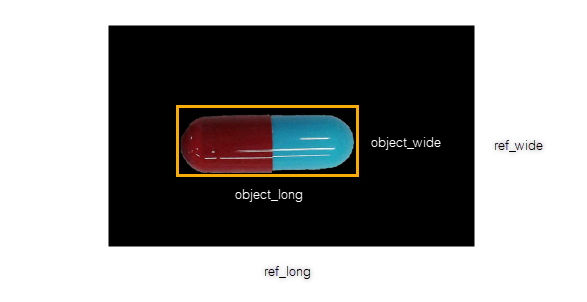
\includegraphics[width=\columnwidth]{Figures/3/opencv3}
			\caption{แสดงการวัดขนาดวัตถุด้วยการใช้วัตถุอ้างอิง}
			\label{Fig:opencv3}
		\end{figure}
		

	\subsection{การหาลักษณะสีของยาเม็ด}
		จากรูปที่ \ref{Fig:opencv3} สามารถตรวจพบ Contour กรอบสี่เหลี่ยมสีเหลือง และการหาลักษณะสีของยาเม็ดจะได้จากการแบ่งพื้นของกรอบออกเป็น 4 ส่วนเท่ากัน และดึงค่าสี BGR ที่จุดพิกเซลตรงกลางของแต่ละส่วนนำไปเปรียบเทียบกับตารางที่ 3.6.5 สีที่มีอยู่ในฐานข้อมูลพิสูจน์เอกลักษณ์ยาเพื่อหาค่าต่าง
		
		% \begin{table}[H]
		% 	\caption{ตารางแสดงรหัสสีจากฐานข้อมูลพิสูจน์เอกลักษณ์ยาเม็ด}
		% 	\label{tab:color-list}				
		% 	\begin{tabular}{c}
		% 		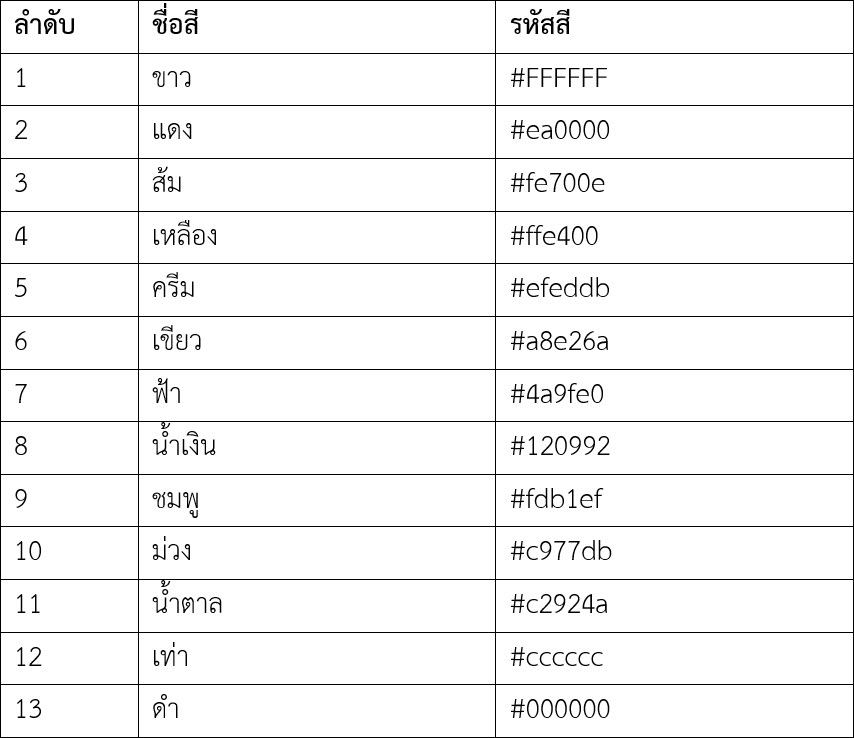
\includegraphics[width=\columnwidth]{Figures/table/color-list}	\\ 
		% 	\end{tabular}
		% \end{table}
		\begin{table}[H]
			\centering
			\caption{ตารางแสดงรหัสสีจากฐานข้อมูลพิสูจน์เอกลักษณ์ยาเม็ด}
			\label{tab:color-list}
			\begin{tabular}{ | c | c | c | }
			\hline
			\textbf{ลำดับ} &	\textbf{ชื่อสี} & \textbf{รหัสสี}  \\ \hline
			1	&	ขาว		&	\#FFFFFF  \\ \hline
			2	&	แดง		&	\#ea0000  \\ \hline
			3	&	ส้ม		&	 \#fe700e \\ \hline
			4	&	เหลือง	& \#ffe400 \\ \hline
			5	&	ครีม	& \#efeddb \\ \hline
			6	&	เขียว	& \#a8e26a \\ \hline
			7	&	ฟ้า		&	\#4a9fe0 \\ \hline
			8	&	น้ำเงิน   &	  \#120992 \\ \hline  
			9	&	ชมพู	& \#fdb1ef \\ \hline
			10	&	ม่วง	& \#c977db	\\ \hline
			11	&	น้ำตาล	& \#c2924a	\\ \hline
			12	&	เท่า	& \#cccccc	\\ \hline
			13	&   ดำ 	  &   \#000000	\\ \hline
			\end{tabular}
		\end{table}
		






